\documentclass{article}
\usepackage{cite} % Add this line to include the cite package for citations

% Language setting
% Replace `english' with e.g. `spanish' to change the document language
\usepackage[english]{babel}

% Set page size and margins
% Replace `letterpaper' with `a4paper' for UK/EU standard size
\usepackage[letterpaper,top=2cm,bottom=2cm,left=3cm,right=3cm,marginparwidth=1.75cm]{geometry}

% Useful packages
\usepackage{amsmath}
\usepackage{graphicx}
\usepackage[colorlinks=true, allcolors=blue]{hyperref}

\title{Journal, Week-1}
\author{Raja Kantheti}

\begin{document}
\maketitle

% \begin{abstract}
% Your abstract.
% \end{abstract}

\section{Introduction}
I am a master's student in Computer Science at UCCS. I want to choose the thesis path to satisfy the degree requirements. My expected course outcomes are to learn what it means to conduct research, how to write scientific papers, better articulate my ideas and evaluate their novelty, and write at least one paper of any type by the end of the semester.

My eagerness to learn and grow is reflected in my goals for this course. I am determined to evaluate my thesis proposal, understand the necessary steps to evaluate the outcomes of my thesis, and grasp the elements of a successful proposal. I am also excited to challenge myself, to see if I have the stamina for long-term research and if this path is the right one for my career progression.

Some personal things about me outside of academia are that I like to be in solitude from time to time, lost in my thoughts and devices, contemplating meta-ethics, talking and debating with myself, and exploring all possibilities. The routines that would allow me to do this are my hobbies: Long walks and longer drives, camping alone, hiking in state/national parks, and this could be well out of the normalcy my other hobbies suggest, wood carving. 
\begin{figure}[h]
\centering
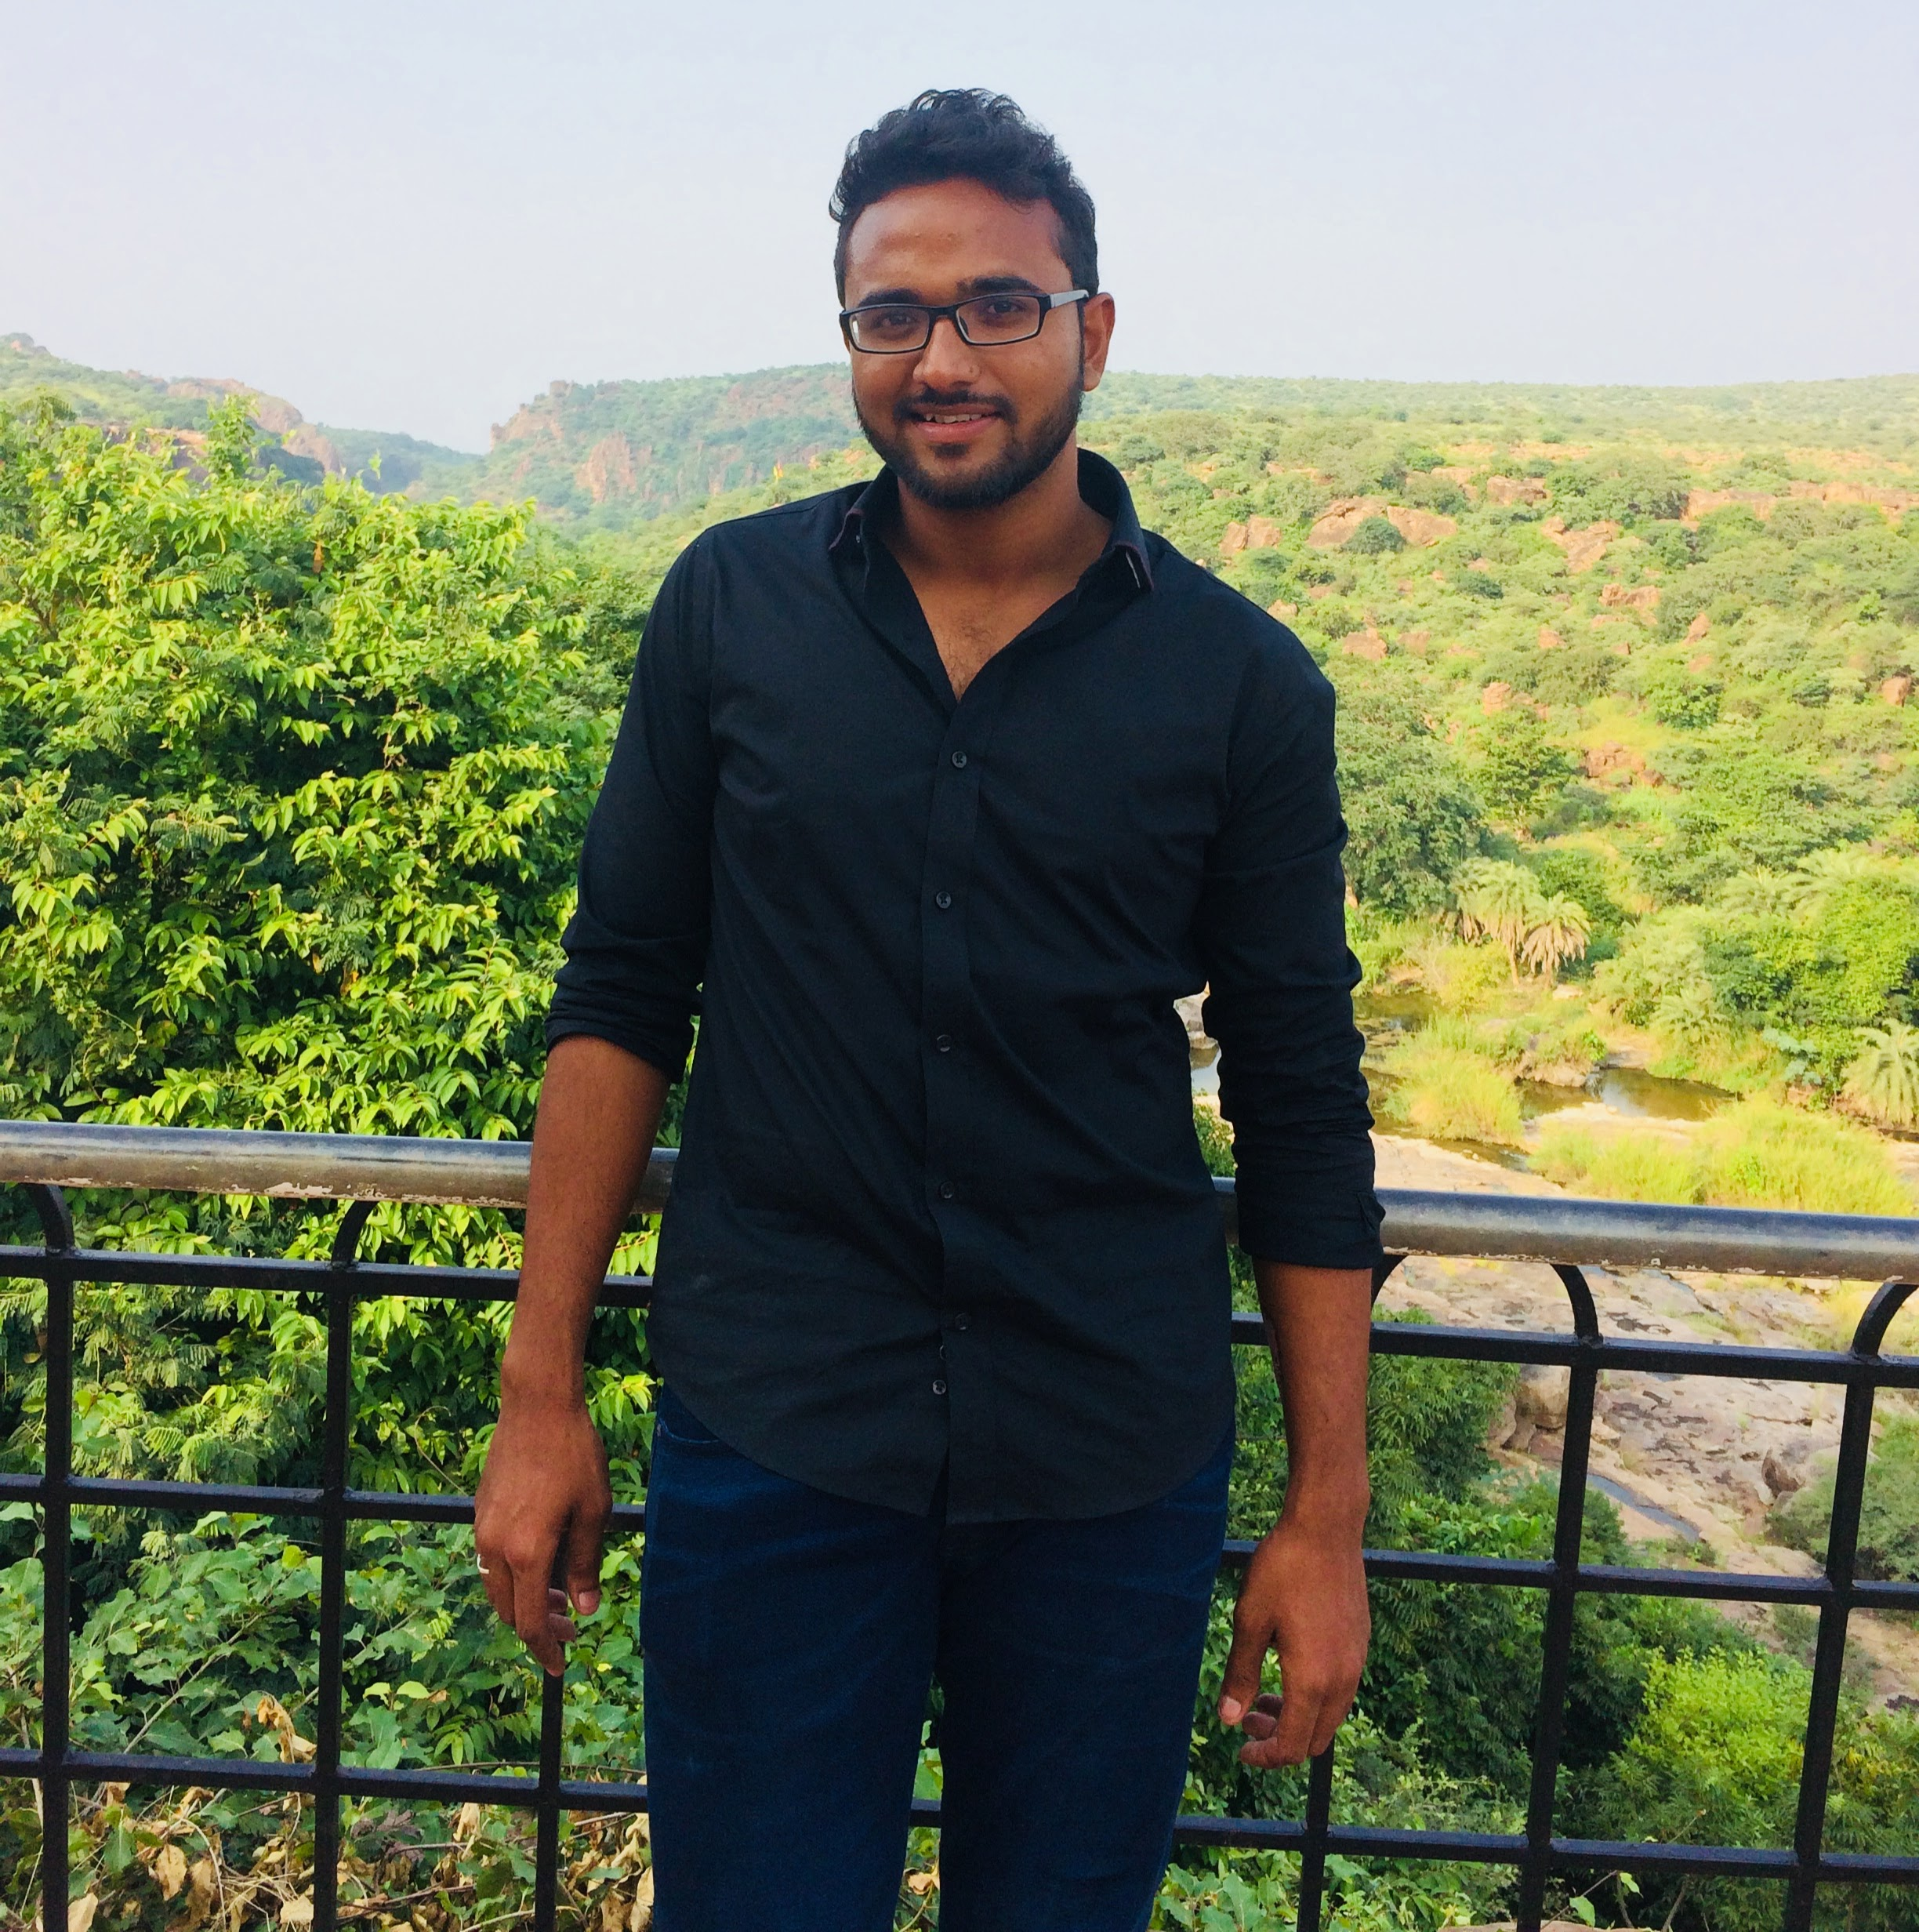
\includegraphics[width=0.25\linewidth]{IMG_1667.JPG}
\caption{'tis I. }
\end{figure}

\subsection[short]{Rationale on what was a good paper}
According to me, a good paper should question and delve into the fundamentals of its field by presenting a novel approach to understanding the core principles of Computer Science. It should provide proof of concept through unbiased experiments that reflect realistic scenarios, ensuring the integrity and applicability of the results. Additionally, the benchmarks or metrics used to quantify the findings must be relevant and appropriate, accurately measuring the impact and significance of the research conducted. 
\section{Tools}
\subsection[short]{}


\end{document}